\begin{enumerate}[label=\thechapter.\arabic*,ref=\thechapter.\theenumi]
\item Consider the signals $x\brak{n}$=$2^{n-1} u\brak{ -n+2}$ and $y\brak{n}$=$2^{-n+2}u\brak{ n+1}$, where $u\brak{n}$ is the unit step sequence. Let $X\brak{e^{j\omega}}$ and $Y\brak{e^{j\omega}}$ be the discrete-time Fourier of $x\brak{n}$ and $y\brak{n}$,respectively. The value of the integral $\frac{1}{2\pi}\int_{0}^{2\pi} X\brak{e^{j\omega}} Y\brak{e^{-j\omega}} d \omega$
(rounded off to one decimal place) is \underline{{\hspace{1.5in}}}\\
\hfill{(GATE EC 41 2021)}\\
\solution
\documentclass[journal,12pt,twocolumn]{IEEEtran}
\usepackage{cite}
\usepackage{amsmath,amssymb,amsfonts,amsthm}
\usepackage{algorithmic}
\usepackage{graphicx}
\usepackage{textcomp}
\usepackage{xcolor}
\usepackage{listings}
\usepackage{enumitem}
\usepackage{mathtools}
\usepackage{gensymb}
\usepackage{comment}
\usepackage[breaklinks=true]{hyperref}
\usepackage{tkz-euclide}
\usepackage{gvv} 
\def\inputGnumericTable{} 
\usepackage[latin1]{inputenc} 
\usepackage{color} 

\newtheorem{theorem}{Theorem}[section]
\newtheorem{problem}{Problem}
\newtheorem{proposition}{Proposition}[section]
\newtheorem{lemma}{Lemma}[section]
\newtheorem{corollary}[theorem]{Corollary}
\newtheorem{example}{Example}[section]
\newtheorem{definition}[problem]{Definition}
\newcommand{\BEQA}{\begin{eqnarray}}
\newcommand{\EEQA}{\end{eqnarray}}
\newcommand{\define}{\stackrel{\triangle}{=}}
\theoremstyle{remark}
\newtheorem{rem}{Remark}

\begin{document}

\bibliographystyle{IEEEtran}
\vspace{3cm}

\title{GATE 2022-IN}
\author{EE23BTECH1205 - Avani Chouhan$^{*}$}
\maketitle
\newpage
\bigskip

\renewcommand{\thefigure}{\theenumi}
\renewcommand{\thetable}{\theenumi}

\vspace{3cm}
\textbf{Question : 18} \\
A signal \( x(t) \) is band-limited between 100 Hz and 200 Hz. A signal \( y(t) \) is related to \( x(t) \) as follows:\\

\( y(t) = x(2t - 5) \)\\
The statement that is always true is \\

\begin{enumerate}
  \item[(A)] \( y(t) \) is band-limited between 50 Hz and 100 Hz
  \item[(B)] \( y(t) \) is band-limited between 100 Hz and 200 Hz
  \item[(C)] \( y(t) \) is band-limited between 200 Hz and 400 Hz
  \item[(D)] \( y(t) \) is not band-limited 
\end{enumerate}

\hfill{(GATE IN 2022)}\\
\textbf{Solution:} \\
\begin{align}
x(t) &\rightleftharpoons X(\omega) \label{eq1}\\
x(at) &\rightleftharpoons \frac{1}{|a|} X\left(\frac{\omega}{a}\right) \label{eq2}\\
x(2t) &\rightleftharpoons \frac{1}{2} X\left(\frac{\omega}{2}\right) \label{eq3}\\
x(t - t_0) &\rightleftharpoons e^{-j\omega t_0}X(\omega) \label{eq4}\\
x(2t - 5) &\rightleftharpoons e^{-j5\omega} \cdot \frac{1}{2} X\left(\frac{\omega}{2}\right) \label{eq5}
\end{align}

The operation \(x(2t-5)\) compresses time by a factor of 2 and shifts 5 units rightward. This expands the frequency domain, doubling the bandwidth of \(x(t)\) from 100 Hz to 200 Hz to \(y(t)\) between 200 Hz and 400 Hz.\\

Hence, the correct answer is option (C).

\end{document}


\pagebreak
\item Consider a continuous-time signal $x\brak{t}$ \,defined by $x\brak{t}=0$\,for $\abs{t}>1$, and $x\brak{t}=1-\abs{t}$ for $\abs{t}\le 1$. Let the Fourier transform of $x\brak{t}$ be defined as $X\brak{\omega}=\int_{-\infty}^{\infty}x\brak{t}e^{-j\omega t} dt$. The maximum magnitude of $X\brak{\omega}$ is $\hbox to 4em{\thinspace\hrulefill\thinspace}$.
\hfill{(GATE 2021 EE 43)}\\
\solution
\iffalse
\let\negmedspace\undefined
\let\negthickspace\undefined
\documentclass[journal,12pt,onecolumn]{IEEEtran}
\usepackage{cite}
\usepackage{amsmath,amssymb,amsfonts,amsthm}
\usepackage{algorithmic}
\usepackage{graphicx}
\usepackage{textcomp}
\usepackage{xcolor}
\usepackage{txfonts}
\usepackage{listings}
\usepackage{enumitem}
\usepackage{mathtools}
\usepackage{gensymb}
\usepackage{comment}
\usepackage{caption}
\usepackage[breaklinks=true]{hyperref}
\usepackage{tkz-euclide} 
\usepackage{listings}
\usepackage{gvv}                                        
\def\inputGnumericTable{}                                 
\usepackage[latin1]{inputenc}                                
\usepackage{color}                                            
\usepackage{array}                                            
\usepackage{longtable}                                       
\usepackage{calc}                                             
\usepackage{multirow}                                         
\usepackage{hhline}                                           
\usepackage{ifthen}                                           
\usepackage{lscape}

\newtheorem{theorem}{Theorem}[section]
\newtheorem{problem}{Problem}
\newtheorem{proposition}{Proposition}[section]
\newtheorem{lemma}{Lemma}[section]
\newtheorem{corollary}[theorem]{Corollary}
\newtheorem{example}{Example}[section]
\newtheorem{definition}[problem]{Definition}
\newcommand{\BEQA}{\begin{eqnarray}}
\newcommand{\EEQA}{\end{eqnarray}}
\newcommand{\define}{\stackrel{\triangle}{=}}
\theoremstyle{remark}
\newtheorem{rem}{Remark}
\begin{document}

\bibliographystyle{IEEEtran}
\vspace{3cm}

\title{GATE 2021 EE 43}
\author{EE23BTECH11022 - G DILIP REDDY}
\maketitle

\bigskip

\renewcommand{\thefigure}{\arabic{figure}}
\renewcommand{\thetable}{\arabic{table}}
\textbf{Question}:\\
Consider a continuous-time signal $x\brak{t}$ \,defined by $x\brak{t}=0$\,for $\abs{t}>1$, and $x\brak{t}=1-\abs{t}$ for $\abs{t}\le 1$. Let the Fourier transform of $x\brak{t}$ be defined as $X\brak{\omega}=\int_{-\infty}^{\infty}x\brak{t}e^{-j\omega t} dt$. The maximum magnitude of $X\brak{\omega}$ is $\hbox to 4em{\thinspace\hrulefill\thinspace}$.
\hfill{(GATE 2021 EE 43)}
\\\\
\solution
\fi
\begin{align}
X\brak{f}&=\int_{-\infty}^{\infty}x\brak{t}e^{-j2\pi f t} dt\\
X\brak{f}&=\int_{-1}^{1}\brak{1-\abs{t}}e^{-j2\pi f t} dt\\
X\brak{f}&=\int_{-1}^{1}e^{-j2\pi f t} 
dt - \int_{-1}^{1}\abs{t}e^{-j2\pi f t} dt\\
X\brak{f}&=2\int_{0}^{1}\cos\brak{{2\pi f t}}
dt - 2\int_{0}^{1}t\cos\brak{2\pi f t} dt\\
X\brak{f}&=2\frac{\sin\brak{{2\pi f }}}{2\pi f}
- 2\sbrak{\frac{\sin\brak{2\pi f }}{2\pi f}+\frac{\cos\brak{2\pi f }}{\brak{2\pi f}^2}-\frac{1}{\brak{2\pi f }^2}}\\
X\brak{f}&=2\frac{1-\cos\brak{2\pi f }}{\brak{2\pi f}^2}\\
X\brak{f}&=2\frac{2\sin^2\brak{\frac{2\pi f}{2}}}{\brak{2\pi f}^2}\\
X\brak{f}&=\frac{\sin^2\brak{\pi f}}{\brak{\pi f}^2}\\
f& \to 0 \implies X\brak{f}\to1
\end{align}
Maximum of magnitude of $X\brak{f}=1$
\begin{figure}[h]
    \centering
    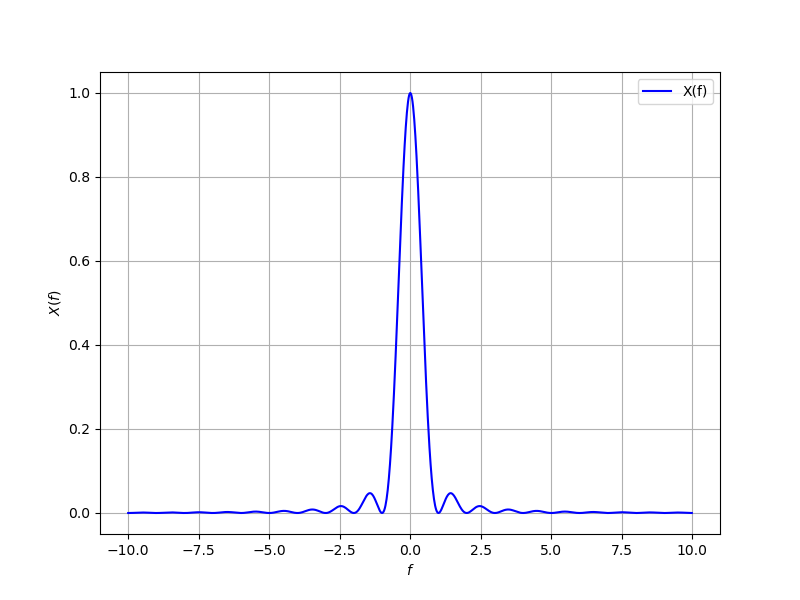
\includegraphics[width=1\linewidth]{2021/EE/43/figs/graph.png}
    \caption{plot of X(f)}
\end{figure}
%\end{document}

\pagebreak
\end{enumerate}
